
\section{The \BaFePAs series}

The \BaFePAs series is one of many that stem from the parent compount \BaFeAs, although unlike the electron doped \BaCoFeAs and the hole doped \BaKFeAs series, the \BaFePAs progression is entirely isovalent meaning that the changes affected due to the P substitution are due to structure and chemical pressure rather than additional charge carriers. Nonetheless, superconductivity occurs with a very similar phase diagram as with the charge-doped examples in the same `$122$' family of iron-pnictide materials.\footnote{See for example \Fig1 in ref.\cite{Paglione2010}}

The \BaFePAs series progresses from \BaFeAs which becomes antiferromagnetic at around \unit[138]{K} towards \BaFeP which is metallic to low temperatures. Neither end members are superconducting, however as As is substituted for P, the low temperature antiferromagnetic state decays, giving way to superconductivity which kicks in at approximately $x=0.18$ and increases to the optimal substitution of $x=0.31$. Superconductivity then decreases until it gives way to a paramagnetic ground state at around $x=0.71$. \Fig\ref{Fig:3:PhaseDiagram} shows the phase diagram adapated from ref. \cite{Nakai2010a} as determined by resistivity measurements.

\begin{figure}
    \begin{center}
        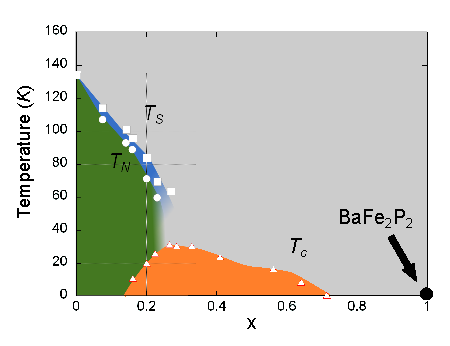
\includegraphics[scale=1.0]{Chapter3-dHvABaFe2P2/Figures/BaFe2P2Series/PhaseDiagram/PhaseDiagram}
        \caption{Phase diagram adapted from ref \cite{Nakai2010a} measured by resistivity. $T_s$, $T_N$ and $T_c$ are the structural transition, the antiferromagnetic transition and the superconducting transition temperatures respectively.}
        \label{Fig:3:PhaseDiagram}
    \end{center}
\end{figure}

 The progression along the series is isovalent since P and As are in the same periodic group (Group $V$ -- the pnictides). The net effect of the substitution is to apply an increasing chemical pressure as $x$ moves towards $1$. Several reports show that applying \textit{physical} pressure to \BaFeAs results in a similar phase diagram with an antiferromagnetic phase and superconductivity up to $\sim$\unit[30]{K}\cite{Yamazaki2010,Colombier2009,Alireza2009} and in Klintberg \textit{et al.}\cite{Klintberg2010} a direct comparison has been made between the two. 

Structurally, the unit cell of the series is tetragonal ($I4/mmm$) for most of the phase diagram, aside from an orthorhombic phase below the $T_s$ line as shown in \fig\ref{Fig:3:PhaseDiagram}. The unit cell $a$ axis shrinks slightly less as pressure is applied compared with the $c$ axis ($\sim3\%$ c.f. $\sim4.5\%$ respectively). Interestingly though the $c$ axis shrinking largely occurs in the Fe-Pnictide plane leading to some theories of the superconductivity emerging from the tetrahedral bond angle between the Fe and the pnictigen. %TODO: ref

\begin{figure}
    \begin{center}
        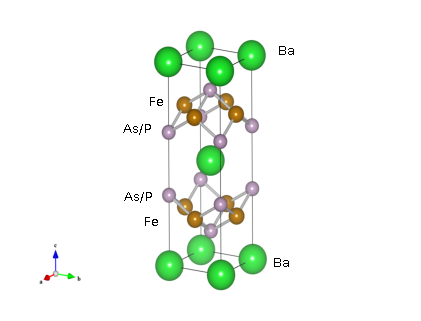
\includegraphics[scale=1.0]{Chapter3-dHvABaFe2P2/Figures/BaFe2P2Series/UnitCell/UnitCell}
        \caption{The tetragonal unit cell of the 122 \BaFePAs series.}
        \label{Fig:3:UnitCell}
    \end{center}
\end{figure}

By measuring the end member of the series, important conclusions can be drawn as to the potential mechanisms of superconductivity in this family of materials.

The \BaFePAs series has been previously measured by members of the group at Bristol using dHvA oscillations\cite{Shishido2010}. As suggested in the Shishido reference, since dHvA has been observed across such a large range of substitutions, it implies that the material is not prone to disorder as is the case in many charge doped series (TODO ref). The electron surfaces have been characterised for x ranging from $0.41$ to $1$ and have clearly shown that the DFT calculations consistently overestimate the size of the surfaces. Moreover, dHvA measurements on the material with $x=0.63$ have been performed where one of the hole surface extrema was observed\cite{Analytis2010c} however DFT calculations as well as comparisons with \SrFeP\cite{Analytis2009} and considerations of compensated Fermi surface volumes give evidence for two hole as well as two electron fermi surfaces for materials towards the P end of the series, (towards the As end of the series, there appears an extra, pinched off, hole surface around the $\Gamma$ point). If the electron Fermi surfaces are oversized in the DFT calculations, then the hole Fermi surface volumes should also be oversized in order to remain compensated. What is not clear though is whether the geometry is altered -- DFT calculations show the larger of the hole pockets undergoing significant changes, specifically in that it becomes much more three dimensional as P substitution becomes more complete. This thesis presents data which elucidates the shape of the outer hole surface.

